\documentclass[3p,times,procedia]{elsarticle}
\flushbottom

\usepackage{ecrc}
\usepackage[bookmarks=false]{hyperref}
    \hypersetup{colorlinks,
      linkcolor=blue,
      citecolor=blue,
      urlcolor=blue}

\volume{00}

\firstpage{1}

\journalname{Procedia Computer Science}

\runauth{Tendikov N., & Rzayeva L.}

\jid{procs}

\usepackage{amssymb}

\usepackage[figuresright]{rotating}

\begin{document}
\begin{frontmatter}

\dochead{The 14th International Conference on Emerging Ubiquitous Systems and Pervasive Networks \\(EUSPN 2023) \\ Workshop Intelligent systems based on Internet of Things Technology (IoT) \\ November 7-9, 2023, Almaty, Kazakhstan
}

\title{Integration of GIS and machine learning analytics into Streamlit application}

\author[a]{Noyan Tendikov\corref{cor1}} 
\author[b]{Leila Rzayeva\corref{cor2}}

\address[a]{Astana IT University, Mangilik El avenue 55/11, Astana, 010000, Kazakhstan}
\address[b]{Astana IT University, Mangilik El avenue 55/11, Astana, 010000, Kazakhstan}

\begin{abstract}
This paper introduces an implementation of different GIS tools into Streamlit application: FCNN Terrain Classification, Earth Engine Dataset Parsing, and GIS Timelapse Animations. This toolkit is integrated with terrain multi-classification models using Fully Convolutional Neural Networks (FCNNs) for imagery data into Streamlit microservices. The proposed methodology involves labeled and unlabeled data collection from ESA WorldCover and Sentinel-2 MSI on the Google Earth Engine, compressing datasets into TFRecords format with 9 diverse terrain types, and handling Google Cloud training computations. The experimental results demonstrate the effectiveness of the CNN-based approach, achieving a tolerable from 60\% up to 80\% accuracy of the model and robust classification performance. The simplicity and efficiency of the proposed method make it suitable for real-world tasks requiring reliable and fast GIS analytics.
\end{abstract}

\begin{keyword}
Geographic Information Systems; Terrain Classification; Machine Learning; Deep Learning; Google Cloud Computing; Streamlit;
\end{keyword}

\cortext[cor1]{Corresponding author. Tel.: +7-777-147-5905.}
\cortext[cor2]{Corresponding author. Tel.: +7-777-533-9169.}
\end{frontmatter}
\email{212281@astanait.edu.kz ; l.rzayeva@astanait.edu.kz}

\section{Introduction}
Geographical data plays a crucial role in our world. The emergence of this trend is clearly correlated with the prevalence of Internet of Things (IoT) devices. These accessories cover a wide range of spheres, including urban analytics, crisis management, land cover mapping, remote sensing, and agricultural or environmental sectors. For instance, the percentage of IoT utilization and integration in business processes and industries can reach up to approximately 30\%, which has an impact on increased productivity with efficiency and autonomy \cite{Safari2021}. However, it is important to note that the raw data from these devices inherently holds limited utility to be applied. Therefore, there needs to be dedicated multiphase Extract Transform Load (ETL) pipelines for the collection and transportation of materials for further high-quality processing. This is the only way to achieve a seamless synergy between IoT and GIS \cite{Xinze2021}. The Figure 1 shows the structure of that workflow with four unique parts: event producers, streaming and storing data, transformation and analytics, information within dashboards. 

\begin{figure}[htbp]
\centering

\includegraphics[width=1\linewidth]{gr1}
\caption{Structure of the IoT-related ETL pipeline for GIS analytics.}
\end{figure}

Firstly, IoT devices ensure undisturbed simultaneous data acquisition and transmission. In this context, reconnaissance drones, telecommunications, specialized satellite systems, as well as locally oriented sensors of environmental parameters (temperature, humidity, air composition, etc.) are widely used. For example, drones, or Unmanned Aerial Vehicles (UAVs), are utilized for specific video recordings of limited territorial clusters at nearby distances. In general, their initial mobility makes it possible to obtain information from various perspectives and points of view that is able to improve the completeness of the picture. The current conflict in Ukraine has clearly demonstrated the importance of visual details from scout drones in determining the combat spots of opponents and the navigation of artillery fires on the battlefield \cite{Kunertova2022}. On the other hand, satellites provide a global and qualitative view of the whole Earth’s surface or over large areas in different spectral ranges and time intervals. It adds to the complexity of working with data material but offers valuable insights into separate terrain types and their characteristics. Secondly, data segments are parsed via a variety of streaming services, like Kafka or Beam, before being further distributed into SQL or NoSQL databases. Thus, it is possible to classify and train machine learning algorithms on it as an efficient automated approach of extracting valuable insights from its vast volumes of data. Thirdly, processed data and analytics become full-fledged useful information, which is delivered to a specific web service for further use by monitoring organizations. Taking this into consideration, the recent waves of wildfires in Russia, Kazakhstan, and Canada have shown the need for early or real-time analytics to prevent incidents and save lives. Furthermore, as demonstrated by innovative research, data analysis holds great promise for anticipating the dynamics of heat consumption in the "smart city" format as well as for optimizing the performance of various preservation services\cite{Omirgaliyev2022}.
\section{Methodology}
\subsection{Structure of the project}
The project consists of three main stages of implementation. Primarily, data was collected from Google Earth Engine Datasets, which store GIS information on Sentinel and ESA satellites or IoT devices. Then, based on this data, terrain classification models were trained on the Google Vertex AI platform. In addition, in order to interact with the user interface, one of the most popular third-party visual libraries in Python for building quick local and web apps for the MLOps pipeline (Machine Learning Operations) called Streamlit was chosen \cite{Wazir2023}. It contains pre-made visual components that can be put together as a constructor. The final build also includes the functions of parsing information from the Google Earth Engine datasets and visualizing data in GIF animations in a specific area using GeoJSON files. Applications can be located on a local device or on a separate host, as well as by containerization in Docker.

\subsection{GIS Data Classifications}
GIS experts distinguish three primary categories of classification: automated, manual, and hybrid (combination of automated with manual) \cite{Horning2004}. Automated types are implemented systematically via supervised (labeled data) and unsupervised (unlabeled data) methods. The research of Al-Ahmadi \cite{Al-Ahmadi2009} was presented about ISODATA unsupervised classification with repeatedly dynamic partitioning and merging of clusters of images for a predefined amount of iterations. It is a more complicated approach than Support Vector Machine (SVM), Random Forest (RF), Decision Trees (DT), and K-Means techniques. They are commonly used for fast executions. For example, methods or models in the RF category can present up to 89\% accuracy for tasks such as identifying agricultural cropland in South Asia based on an open Google Earth dataset \cite{Gumma2019}. On top of that, Duro et al. \cite{Duro2012} compared pixel-based and object-based datasets of SPOT-5 HRG and found that trained RF and SVM machine learning models are able to get the same results in the case of accuracy of agricultural landscape recognition, which is over 90\% for both cases. However, machine learning models are limited to the initial augmented data and cannot be applied globally. According to the research of Regan et al.\cite{Bhatnagar2020}, deep learning architectures based on CNNs connections are able to identify different visual figures from large datasets. It is shown that some parameters can be combined in multiple layers in order to make more complicated models, such as VGGNet, ResNet50, SegNet, U-Net, PSPNet, and others. For example, Jeppesen et al. \cite{Jeppesen2019} demonstrated that the implementation of RS-Net (a modified version of U-Net) for the Landsat 8 dataset could detect cloud patterns in less than 34 seconds per image product. In addition, in the research of Zhang et al. \cite{Zhang2018}, it was shown that a patch-based CNN model that is trained on the same Landsat dataset is able to get an overall accuracy of 97\% in the task of only detecting rice plantations near rivers in the China region. This brought us a final, solid understanding that CNN-type models are absolutely required in the project.

\subsection{Dataset Evaluation}
As a means of developing testing and training data collections, two large datasets have been selected from European Space Agency (ESA) satellites: Sentinel-2 MSI and ESA WorldCover. They are available completely free to download from the Google Earth Engine servers or upon request from their API \cite{Bennett2020}. Sentinel-2 consists of a constellation of satellites that constantly provide high-resolution optical imagery of the Earth's surface within 5 to 10 days \cite{Phiri2020}. This dataset is frequently used by governmental or private organizations to plan urban and agricultural monitoring. Although MSI means that it as well consists of multiple spectral ranges, the train data is implemented using only RGB human-visible planes. On the other hand, ESA WorldCover is based on Sentinel-2 and Sentinel-1 data with 10 meters of resolution per pixel. Its products have 11 terrain cover classifications, including "Tree cover", "Grass land", "Built-up", etc. Firstly, in this project, the merging of these two datasets was practiced. ESA WorldCover was used for primary labeling of data regions, but types of classification were limited to 9 amounts: "Water", "Trees", "Grass", "Flooded Vegetation,", "Croups, "Shrub and scrub", "Built-up Areas,", "Bare Ground,", "Snow and Ice.". However, ESA WorldCover consists only of land cover data, so missed values for ocean regions were filled with the "Water" class. Secondly, there are applied Google Cloud Services, which optimize work with data and allow it to be stored or processed in a dedicated bucket. Google Cloud Dataflow with Apache Beam constructs a pipeline for dataset creation by creating shapes of regions in Google Earth Engine and getting sample point examples. There are only a few significant continents or regions of the world represented in this sample, including Europe, Asia, Africa, Australia, North America, and South America. Thirdly, Apache Beam compresses numpy arrays into a single TensorFlow Record. Therefore, for the project, three different datasets were prepared: large (over 1 gigabyte), medium (around 200 megabytes), and small (around 10 megabytes). The final size depends on sampling parameters such as region size or amounts, types of categories, stratification, normalization, and so on.

\subsection{Model Architecture and Training}
In this case, the TensorFlow Keras Python library was utilized to design and implement the FCNN model. It contains various prebuilt patterns for neural networks and deep learning. So, Keras greatly simplifies the implementation of the project by combining diverse structures and APIs. The structure of the final model contains an input layer, a normalization or preprocessing layer, convolutional with deconvolutional layers, and an output layer. All the previously listed layers are fully connected. It means that they connect all the neurons or parameters from the previous layer to another subsequent layer, facilitating complex relationships. Firstly, the input layer receives a dense tensor of information formed from patch size (vertical and horizontal) and number of bands (Sentinel-2 MSI has only 13 of them). This layer does not transform data into any formats. Secondly, the preprocessing layer is an additional layer that standardizes or normalizes the inputs of the initial training dataset in order to improve stability and prevent the dominance of several features. Thirdly, convolutional layers are responsible for capturing local features that detect imagery patterns. They classify pixels step by step around any kernel with some padding around it. Finally, the output layer is based on the idea of activation functions. This function is able to output specific values when a certain neuron threshold is exceeded. The values are given in the format of the multi-class classification distribution of labels. Models were trained on the basis of Google Vertex AI through interaction with the API in Google Colab. Google Vertex AI is known as the leading platform for automating machine learning and model deployment, which greatly simplifies the scaling process \cite{Berg2022}. For this project, a separate dedicated Auto-ML custom container from Google was used with the following characteristics: Container - europe-docker.pkg.dev, CPU - e2-standard-8. During this training process, Adam optimization technique repeatedly updates the parameters of the model. It is practiced for the minimization of a defined loss function, or cross-entropy loss. As a result, there were trained three terrain classification models (TCM): TCM-Large, TCM-Medium, and TCM-Small.

\subsection{Evaluation metrics}
As a way of checking the results of the models, various visual and mathematical indicators are used. In this case, only the main ones were applied that are applied in the evaluation of a classification or prediction model, namely precision, recall, F1 score, and accuracy. Firstly, precision and recall are basic values that show ratios between positive and negative predictions. Secondly, the F1-Score shows balance between precision and recall using their harmonic mean. Lastly, accuracy measures overall correctness by dividing true positives and true negatives by total instances.

\begin{equation}
\begin{aligned}
  Precision &= \frac{TP}{TP+FP}, & \quad Recall &= \frac{TP}{TP+FN} \\
\end{aligned}
\end{equation}

\begin{equation}
\begin{aligned}
  F1 &= \frac{2 \cdot Precision \cdot Recall}{Precision + Recall}, & \quad Accuracy &= \frac{TP+TN}{TP+TN+FP+FN}
\end{aligned}
\end{equation}

\section{Results and Discussions}
\subsection{FCNN Models}
According to the results of training three models with a different number of epochs, and the size of the training data, the trend is clearly visible that TCM-Large shows the best results. For visual analysis in the Figure 2, here is an urbanized region in Astana city of Kazakhstan that has a combination of many details of vegetation, water, and buildings. TCM-Large displays agile and more obvious distributions of areas with an accurate classification by region and type. Furthermore, it demonstrated "relatively" acceptable indicators of qualities: average precision - 0.67, recall - 0.71, f1-score - 0.65, accuracy - 0.71. It can be seen from the sampling results in Table 1.

\begin{figure}[htbp]
\centering
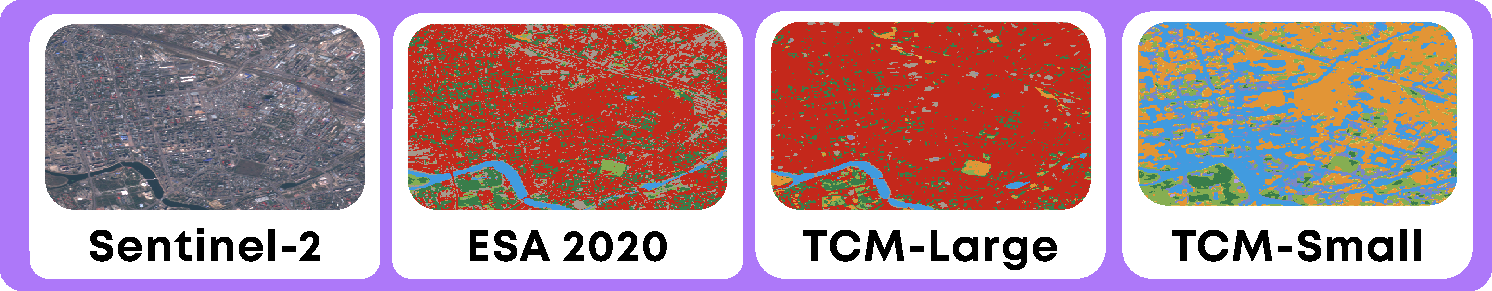
\includegraphics[width=1\linewidth]{gr2}
\caption{Visual predictions comparison of models (2020 - 2021 years, lat. - 51.172, long. 71.438, pixels - 512x512, scale - 10 meter/pixel).}
\end{figure}

\begin{table}[h]
\caption{Precision, accuracy, recall, f1-score of TCM models.}
\begin{tabular*}{\hsize}{@{\extracolsep{\fill}}llll@{}}
\toprule
Models & Precision ({\it{t}}) & Recall ({\it{t}}) & F-Score ({\it{t}}) \\
\colrule
TCM-Large (macro avg) & 0.38 & 0.32 & 0.32\\
TCM-Large (weighted avg) & 0.67 & 0.71 & 0.65\\
TCM-Small (macro avg) & 0.23 & 0.44 & 0.06\\
TCM-Small (weighted avg) & 0.78 & 0.06 & 0.05\\
\botrule
TCM-Large (accuracy) & & & \textbf{0.71}\\
TCM-Small (accuracy) & & & \textbf{0.06}\\
\botrule
\end{tabular*}
\end{table}

As a result, indicators suggest that the TCM-Large might be suitable for simplified and rapid territorial analysis, as demonstrated in the Table 2. On the other hand, the experimental model TCM-Small showed substandard results in the form of accuracy - 0.06 for obvious reasons.

\begin{table}[h]
\caption{Calculated processing time per product of the TCM-Large model.}
\begin{tabular*}{\hsize}{@{\extracolsep{\fill}}lllll@{}}
\toprule
\textbf{Scale / Resolution} & \textbf{128px} & \textbf{256px} & \textbf{512px} & \textbf{800px}\\
\colrule
10 meters & 0.077s & 0.110s & 0.242s & 1.515s\\
20 meters & 0.085s & 0.231s & 0.287s & 1.618s\\
80 meters & 0.124s & 0.263s & 0.324s & 1.670s\\
\botrule
Average & 0.095s & 0.201s & 0.284s & 1.601s\\
Median & 0.085s & 0.231s & 0.287s & 1.618s\\
\botrule
\end{tabular*}
\end{table}

\begin{figure}[htbp]
\centering
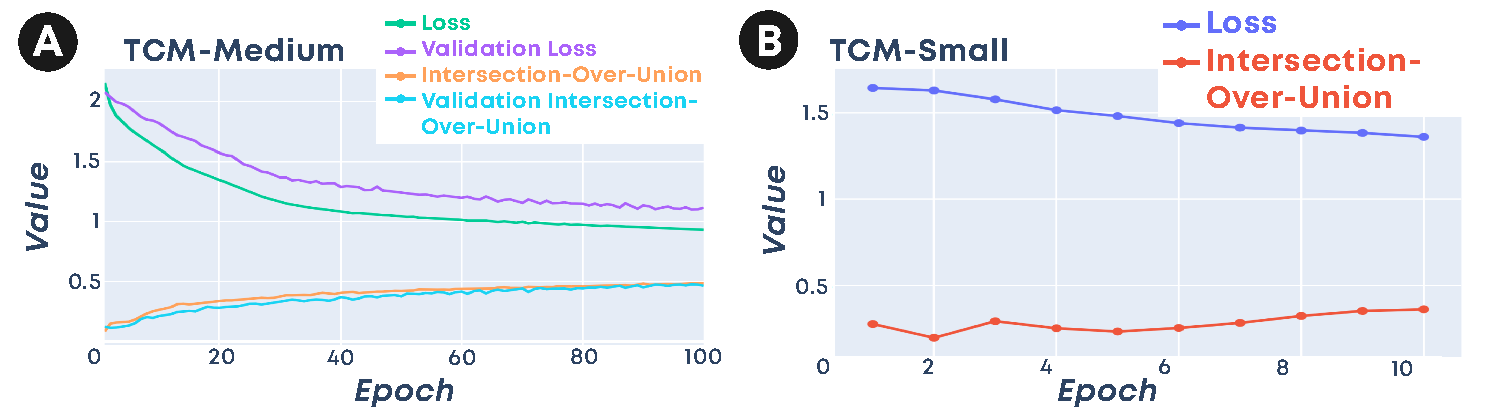
\includegraphics[width=1\linewidth]{gr3}
\caption{Training results of TCM-Small and TCM-Large models.}
\end{figure}

Because of the special allocation of the smallest possible dataset for this model and the number of training epochs was limited to only 10, not 100 like in other larger models, as shown in the Figure 3. The learning process was compared in terms of training loss and validation loss. Additionally, there was applied the Intersection-Over-Union test metric which allows us to see the overlay metric of segmentation masks. The larger this indicator, the better the process of overlaying and classification in the model. Thus, the trend is clear that models do not provide sharp progress and results in the learning process, even though the association between val and loss is basically valid. Although these observations suggest the absence of clear indications of overfitting or underfitting tendencies within the models, the training process lacks pronounced improvements. It points towards potential challenges in model performance and optimization. Further analysis and investigation are necessary to identify and address the factors contributing to this phenomenon.

\subsection{Practical standpoint and additional toolkit}
The Figure 4 (a) shows the interface of this application based on the TCM-Large model, in which there is a choice of location by name and coordinates, date frames, patch size, and image scale. Scale contributes to "compressing" the image so that it displays more or less meters per pixel. Its default is 10 meters per pixel. On the contrary, the patch size is potentially unlimited, but the Google Cloud API does not allow sending too much data and limits traffic for individual accounts. In any case, a value of 512 is optimal, while 800 is a probable limit per data request. Last but not least, here is the result of the predictions with detailed statistics of visual and analytics results per class in the Figure 4 (b, c). Additionally, there are supplementary GIS functionalities and other tools for timelapses with a detailed setting of time limits and region selection. The Earth Engine Datasets page works on the same principle of parsing data from Google.

\begin{figure}[htbp]
\centering
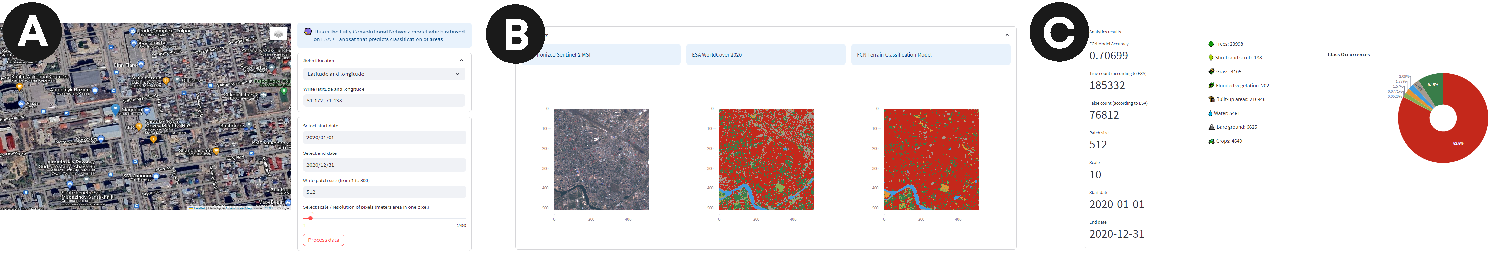
\includegraphics[width=1\linewidth]{gr4}
\caption{(a) Input GIS data; (b) Visual results of the model; (c) Analytics results of the model.}
\end{figure}

\section{Conclusion}
This research paper was aimed at trying to simplify the creation of a GIS analytics Streamlit application with competent terrain classification models based on FCNN and satellite information. By leveraging the power of data from ESA satellites, we have achieved minor-to-average results. However, it should be noted that the FCNN structure is not enough to conduct large-scale studies. It is only suitable for simplified and rapid territorial analysis. Therefore, it needs to combine the architecture of the model with alternative approaches such as U-Net or improve the learning process and the quality of the model. The further development of the project should also focus on creating custom IoT devices for data collection and processing rather than relying on pre-existing datasets. Also, there would be an expansion of the functional possibilities of machine learning models and switching to another FastAPI or Django framework architecture to improve the security structure.

\begin{thebibliography}{}
\bibitem{Safari2021}
Safari, B. J., Sadeghi-Niaraki, A., and Choi, S.-M. (2021) ''A Survey of GIS and IoT Integration: Applications and Architecture." {\it Applied Sciences}. {\bf 11} (21): 10365. doi: 10.3390/app112110365.
\bibitem{Xinze2021}
Xinze, L., and Baixi, Z. (2021) ''An automated data engineering pipeline for anomaly detection of IoT sensor data." {\it Cornell University}. doi: 10.3929/ethz-b-000584078.
\bibitem{Kunertova2022}
Kunertova, D. (2022) ``The Ukraine Drone Effect on European Militaries." {\it  Center for Security Studies}. {\bf 10} (15): 1--4. doi: 10.3929/ethz-b-000584078.
\bibitem{Omirgaliyev2022}
Omirgaliyev, R., Zhakiyev, N., Aitbayeva, N., Akhmetbekov, Y. (2022) ``Application of machine learning methods for the analysis of heat energy consumption by zones with a change in outdoor temperature: Case study for Nur-Sultan city." {\it  International Journal of Sustainable Development and Planning}. {\bf 17} (4): 1247--1257. doi: 10.18280/ijsdp.170423.
\bibitem{Wazir2023}
Wazir, S., Kashyap, G. S., and Saxena, P. (2023) ``MLOps: A review" {\it  Cornell University}. doi: 10.48550/arxiv.2308.10908.
\bibitem{Horning2004}
Horning, N. (2004) ``Land cover classification methods." {\it American Museum of Natural History, Center for Biodiversity and Conservation}. http://biodiversityinformatics.amnh.org.
\bibitem{Al-Ahmadi2009}
Al-Ahmadi, F. and Hames, A. (2009) ``Comparison of Four Classification Methods to Extract Land Use and Land Cover from Raw Satellite Images for Some Remote Arid Areas, Kingdom of Saudi Arabia." {\it Journal of King Abdulaziz University-Earth Sciences}. {\bf 20} (1): 167--191. doi: 10.4197/ear.20-1.9.
\bibitem{Gumma2019}
Gumma, M. K., Thenkabail, P. S., Teluguntla, P., Oliphant, A., Xiong, J., Giri, C., Pyla, V., Dixit, S., and Whitbread, A. (2019) ``Agricultural cropland extent and areas of South Asia derived using Landsat satellite 30-m time-series big-data using random forest machine learning algorithms on the Google Earth Engine cloud." {\it Giscience & Remote Sensing}. {\bf 57} (3): 302--322. doi: 10.1080/15481603.2019.1690780.
\bibitem{Duro2012}
Duro, D. C., Franklin, S. E., and Dubé, M. G. (2012) ``A comparison of pixel-based and object-based image analysis with selected machine learning algorithms for the classification of agricultural landscapes using SPOT-5 HRG imagery." {\it Remote Sensing of Environment}. {\bf 118}: 259--272. doi: 10.1016/j.rse.2011.11.020.
\bibitem{Bhatnagar2020}
Bhatnagar, S., Gill, L., and Ghosh, B. (2020) ``Drone image segmentation using machine and deep learning for mapping raised bog vegetation communities." {\it Remote Sensing}. {\bf 12} (16): 2602. doi: 10.3390/rs12162602.
\bibitem{Jeppesen2019}
Jeppesen, J., Jacobsen, R. H., Inceoglu, F., and Toftegaard, T. S. (2019) ``A cloud detection algorithm for satellite imagery based on deep learning." {\it Remote Sensing of Environment}. {\bf 229}: 247--259. doi: 10.1016/j.rse.2019.03.039.
\bibitem{Zhang2018}
Zhang, M., Lin, H., Wang, G., Sun, H., and Fu, J. (2018) ``Mapping Paddy Rice Using a Convolutional Neural Network (CNN) with Landsat 8 Datasets in the Dongting Lake Area, China." {\it Remote Sensing}. {\bf 10} (11): 1840. doi: 10.3390/rs10111840.
\bibitem{Bennett2020}
Bennett, M. K., Younes, N., and Joyce, K. E. (2020) ``Automating drone image processing to map coral reef substrates using Google Earth Engine." {\it Drones}. {\bf 4} (3): 50. doi: 10.3390/drones4030050.
\bibitem{Phiri2020}
Phiri, D., Simwanda, M., Salekin, S., Nyirenda, V. R., Murayama, Y., and Ranagalage, M. (2020) ``Sentinel-2 Data for Land Cover/Use Mapping: A Review." {\it Remote Sensing}. {\bf 12} (14): 2291. doi: 10.3390/rs12142291.
\bibitem{Berg2022}
Berg, G. (2022). ``Image Classification with Machine Learning as a Service: - A comparison between Azure, SageMaker, and Vertex AI." {\it Diva Portal}.

\end{thebibliography}

\end{document}